\section{What is plasticity and how to measure that}

~ Half page write-up
\begin{itemize}
    \item Explain the literature and their evaluation metrics (as Eq?)
    \item Explain what we would consider
    \item Methods to reduce LoP - l2 reg, layer norm, crelu etc.
\end{itemize}


--> mention that we only look at training in this scenario not test or validation and this is different from catastrophic forgetting 

Example exp \autoref{fig:cnn_example}:
\begin{itemize}
    \item the following CIFAR10 exp shows loss of plasticity when ...
    \item Show lop in terms of evaluation metric
    \item Show how methods like L2, layer norm help reduce LoP.
\end{itemize}
\begin{figure}[t]
    \centering
    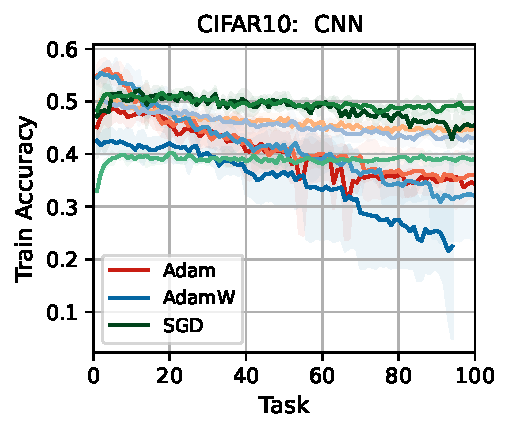
\includegraphics[width=\linewidth]{figs/Accuracy/image/cnn/cifar10_50.pdf}
    \caption{Accuracy of different models on CIFAR10.}
    \label{fig:cnn_example}
\end{figure}
